% vim: set tw=0:
\documentclass{beamer}
\usepackage{graphicx}
\usepackage{booktabs}

% Reasonable themes:
% Antibes Bergen Berkeley Berlin Frankfurt Goettingen Ilmenau Luebeck Malmoe
% Montpellier PaloAlto Rochester Singapore Szeged Warsaw bars boxes
% compatibility default lined plain shadow sidebar split tree
% And these ones include the author's name on every slide:
% Berkeley

% Declare themes.
\mode<presentation>
\usetheme{UWHEP}

% Personal macros.
\newcommand{\email}[1]{{\texttt #1}}
\newcommand{\newframe}[1]{\section{#1}
    \frametitle{\sc{#1}}}
\newcommand{\subframe}[1]{\subsection{#1}
    \frametitle{\sc{#1}}}
\newcommand{\supers}[1]{\ensuremath{^\textrm{#1}}}
\newcommand{\subs}[1]{\ensuremath{_\textrm{#1}}}
\newcommand{\ca}{\ensuremath{\sim}}

% Author information.
\title{Site report: Wisconsin}
\author[Maier, Mohapatra]{
    Will Maier \and Ajit Mohapatra\\ 
    {\tt wcmaier@hep.wisc.edu}\\
    {\tt ajit@hep.wisc.edu}}
\institute[Wisconsin]{University of Wisconsin - High Energy Physics}
\date[2008.04.11]{USCMS T2 Workshop - Purdue, 2008.04.11}
\logo{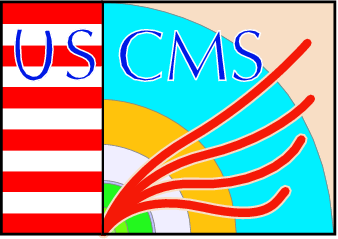
\includegraphics[height=0.6cm]{../../../Graphics/USCMS_logo.png}\hspace{.1cm}
\includegraphics[height=0.75cm]{../../../Graphics/UW_logo.png}}

\begin{document}

% Notes:
%Guidelines for site reports:  What are your plans for completing
%hardware deployment in 2008?  Describe site commissioning status,
%and your experience in getting there.  Describe what expectations
%you think your local or regional community has of you.
%
%OTHER:
%    * condor upgrades
%
%* Hardware commissioning (now vs future)
%    * KSI2K (nodes, CPUs)
%    * TB dCache (disk)
%    * Network (wires)
%    * Site (HVAC)
%* Site commissioning status/experience (what've we done to improve)
%    * SAM
%        * stageout: dCache
%            * aggressive replication policy
%            * new server hardware (PNFS, etc)
%            * new monitoring
%            * debugging
%        * software installation
%            * rerouted CMSSW install jobs to dedicated slots
%
%    * JR
%        * Correct advertisement to RB/DBS (via DBII)
%        * Presence of datasamples
%        * Jobs function (condor, dcache r/w?)
%    * PhEDEx
%        * Links
%* Regional/local community expectations
%    * HLT validation (incl .eu physicists)
%    * Local students (4x) running jobs: Photon jets, Electroweak,
%      QCD


\begin{frame}
    \titlepage
\end{frame}

\section{Overview}
\begin{frame}
    \tableofcontents
\end{frame}

\section{2008 Hardware Deployment}
\subsection{Storage}
\begin{frame}
\begin{itemize}
    \item Through 2007 - 2008, purchased 500 G - 750 G SATA disks
    \item Added disk to integrated UW Plasma cluster
    \item No plans for more dedicated storage
    \item New in 2008: 128 TB on 32 1U servers (1 TB SATA disks)
\end{itemize}

\begin{columns}
\column{2.5in}
\begin{table}
    \begin{tabular}{lr}
        \toprule
        Dedicated dCache & 45 TB \\
        dCache + Condor & 78 TB \\
        \midrule
        Raw & 123 TB \\
        Replicated & 80 TB \\
        \bottomrule
    \end{tabular}
    \caption{2007 Storage Status}
    \label{2007_storage_status}
\end{table}

\column{2.5in}
\begin{table}
    \begin{tabular}{lr}
        \toprule
        Dedicated dCache & 45 TB \\
        dCache + Condor & MM TB \\
        \midrule
        Raw & XX TB \\
        Replicated & ZZ \\
        \bottomrule
    \end{tabular}
    \caption{2008 Storage Status}
    \label{2008_storage_status}
\end{table}

\end{columns}
\end{frame}

\subsection{Compute Resources}
\begin{frame}
\begin{itemize}
    \item All compute nodes upgraded to SL4
    \item Integrated 24 nodes UW Plasma, 32 new dual/quad Xeons
    \item Opportunistic access to FIXME \ca{}1.7k opportunistic GLOW CPUs
    \item New in 2008: 256 CPUs @ 3.0 GHz Xeon on 32 1U servers
\end{itemize}
\begin{columns}
\column{2.5in}
\begin{table}
    \begin{tabular}{lr}
        \toprule
        CPU Class           & KSI2K \\
        \midrule
        2 x 2.4 GHz Xeon    & 64.80 \\    % g3
        2 x 2.8 GHz Xeon    & 158.6 \\    % g4, g5, g6
        2 x 3.0 GHz Xeon    & 99.2 \\     % g7, g8
        4 x 1.8 GHz Opteron & 207.0 \\    % g9 (g10 still Plasma)
        \midrule
        Total & 529.6 \\
        \bottomrule
    \end{tabular}
    \caption{2007 Batch Status}
    \label{2007_Batch_status}
\end{table}

\column{2.5in}
\begin{table}
    \begin{tabular}{lr}
        \toprule
        CPU Class           & KSI2K \\
        \midrule
        2 x 2.4 GHz Xeon    & 64.80 \\    % g3
        2 x 2.8 GHz Xeon    & 158.6 \\    % g4, g5, g6
        2 x 3.0 GHz Xeon    & 99.2 \\     % g7, g8
        4 x 1.8 GHz Opteron & 317.0 \\    % g9, g10
        8 x g12 Xeon & NNN \\             % g12
        \midrule
        Total & XX \\
        \bottomrule
    \end{tabular}
    \caption{2008 Batch Status}
    \label{2008_Batch_status}
\end{table}
\end{columns}
\end{frame}

\subsection{Network}
\begin{frame}
\begin{itemize}
    \item FIXME: chart?
    \item Link to FNAL/Startap
    \item Max observed
\end{itemize}
\end{frame}

\section{Site Commissioning}
\subsection{Storage}
\begin{frame}
\begin{itemize}
    \item blah
\end{itemize}
\end{frame}

\subsection{Compute Resources}
\begin{frame}
\end{frame}

\subsection{Network}
\begin{frame}
\end{frame}

\section{Community Expectations}
\subsection{HLT Validation}
\begin{frame}
\end{frame}

\subsection{Local Students}
\begin{frame}
\begin{itemize}
    \item Photon jets
    \item Electroweak
    \item QCD
\end{itemize}
\end{frame}

\end{document}
